%Given $\Pi_{MAC}$ = (Gen, Enc, Ver)\\

% \begin{center}
%     $ t \leftarrow c = Enc(k,m) $ 
% \end{center}

%To prove by reduction as in Figure \ref{Reduction}
%
%\begin{figure}[h]
%    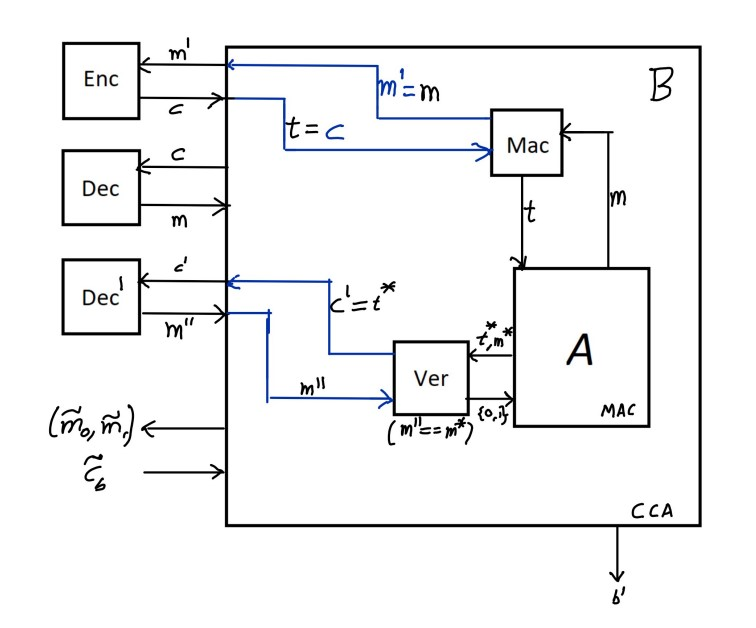
\includegraphics[width=\textwidth,height=\textheight,keepaspectratio]{8-1.jpg}
%    \caption{Proof by Reduction}
%    \label[figure]{Reduction}
%    \centering
%\end{figure}

Lets assume towards contradiction that the MAC construction is not secure $\Rightarrow$ Probablity of forging
this construction $\Pi_{MAC}$ is a non negligible function:

\begin{center}
    $Pr[MacForge_{A,\Pi_{MAC}} = 1] \leq \epsilon(\lambda)$
\end{center}
where $\epsilon(\lambda)$ is a non negligible function.\\


That implies there exists an efficient adversary, A, able to generate a new message and tag pair $(m^*, t^*)$
such that $m^* \notin Q $, and $Ver_k(m^*, t^*) == 1$ with a probablity $\epsilon(\lambda)$. 
% As per the reduction, Ver uses the Dec by comparing $m^*$ with the message from Dec as shown in the Figure \ref*{Reduction}. 
\newline

% Let ValidQuery be the event that B submits a new $(c', t')$ to its
% decryption oracle, Dec' without querying to Enc


% A MAC fogery is only possible when the $m*$ is not queried before and $t*$ should
% be a valid. There exists a distinguisher 

% That means there exits an Adversary, A' able to use the decryption oracel Dec'
% with a new valid tag, $t^*$ and get the message $m''$ and distuingush with  $m^*$ with a probablity $ 1/2 + \epsilon(\lambda)$


% \begin{align}
%     % Pr[ PrivK_{A,\Pi}(\lambda) = 1  \wedge \overline{ValidQuery}]  \leq \epsilon(\lambda)
%      Pr[ PrivK_{A',\Pi}(\lambda) = 1 ] = 1/2 + \epsilon(\lambda)
%     \label{eq1}
% \end{align}

% That implies
% \begin{align}
%     % Pr[ PrivK_{A,\Pi}(\lambda) = 1  \wedge \overline{ValidQuery}]  \leq \epsilon(\lambda)
%     Pr[ PrivK_{A,\Pi}(\lambda) = 1 ]  \leq \epsilon(\lambda)
%     \label{eq1}
% \end{align}
% where $\epsilon(\lambda)$ is a non negligible function.\\



% But given that $\Pi$ is a CCA secure enryption scheme. So
% \begin{align}
%     % Pr[ PrivK_{A,\Pi}^{CCA}(\lambda) = 1  \wedge \overline{ValidQuery}]  \leq 1/2 + neg(\lambda)
%     Pr[ PrivK_{A',\Pi}^{CCA}(\lambda) = 1]  \leq 1/2 + neg(\lambda)
%     \label{eq2}
% \end{align}
% where $neg(\lambda)$ is a negligible function. 


% Equation (\ref*{eq1}) and (\ref*{eq2}) are contradecting to each other as our assumtion 
% that $\epsilon(\lambda)$ is not a negligible is false.


We now consider \(\mathcal{B}\) attacking the CCA-securitv. \(\mathcal{B}\) runs \(\mathcal{A}\) as subroutine. \(\mathcal{B}\) only forward all encryption queries that \(\mathcal{A}\) asks for to his own encryption oracle. Finally \(\mathcal{A}\) outputs a message-tag-pair \(m^*, t^*\). \(\mathcal{B}\) then chooses two messages, lets 
say $\widetilde{m_0}$ as $m^*$ and $\widetilde{m_1}$ as any other random message. If \(\mathcal{B}\) gets the tag $t^*$ as \(\widetilde{c_b}\), it corresponds to $m_0 = m^*$ otherwise it correponds to random message $m_1$. This holds, because \(Dec_k(t) = m \Leftrightarrow Enc_k(m) = t\).\\
\(\mathcal{B}\) is efficient because it only forwards messages, which are of polynomial length (because \(\mathcal{A}\) is efficient), chooses a random number and invokes \(\mathcal{A}\). 
Because \(\mathcal{A}\) can break the MAC with non-negligible probability $\epsilon(\lambda)$ and \(\mathcal{B}\) uses this in every case, \(\mathcal{B}\) can break the CCA security also with non-negligible probability $\epsilon(\lambda)$. 
%So here the success probablity of B is,
%\begin{align}
%    Pr[ PrivK_{B,\Pi'}^{CCA}(\lambda) = 1] \leq |(1 - \epsilon(\lambda))/2|
%    \label{eq1}
%\end{align}
%
%But given that $\Pi$ is a CCA secure enryption scheme. So for CCA secure Adversary A',
%\begin{align}
%    Pr[ PrivK_{A',\Pi}^{CCA}(\lambda) = 1]  \leq 1/2 + neg(\lambda)
%    \label{eq2}
%\end{align}
%where $neg(\lambda)$ is a negligible function. \\
%
%Both equations (\ref*{eq1}) and (\ref*{eq2}) are valid only when
%unless $\epsilon(\lambda)$ is a negligible function which is contradiction to 
%our assumption. 
Because this a contradiction to the CCA security of \(\Pi\), our assumption that such an adversary \(\mathcal{A}\) against the collision resistance of \(\Pi_{MAC}\) exists, is false. 
So \(\Pi_{MAC}\) is a collision resistant MAC.
